% Options for packages loaded elsewhere
\PassOptionsToPackage{unicode}{hyperref}
\PassOptionsToPackage{hyphens}{url}
%
\documentclass[
  ignorenonframetext,
]{beamer}
\usepackage{pgfpages}
\setbeamertemplate{caption}[numbered]
\setbeamertemplate{caption label separator}{: }
\setbeamercolor{caption name}{fg=normal text.fg}
\beamertemplatenavigationsymbolsempty
% Prevent slide breaks in the middle of a paragraph
\widowpenalties 1 10000
\raggedbottom
\setbeamertemplate{part page}{
  \centering
  \begin{beamercolorbox}[sep=16pt,center]{part title}
    \usebeamerfont{part title}\insertpart\par
  \end{beamercolorbox}
}
\setbeamertemplate{section page}{
  \centering
  \begin{beamercolorbox}[sep=12pt,center]{part title}
    \usebeamerfont{section title}\insertsection\par
  \end{beamercolorbox}
}
\setbeamertemplate{subsection page}{
  \centering
  \begin{beamercolorbox}[sep=8pt,center]{part title}
    \usebeamerfont{subsection title}\insertsubsection\par
  \end{beamercolorbox}
}
\AtBeginPart{
  \frame{\partpage}
}
\AtBeginSection{
  \ifbibliography
  \else
    \frame{\sectionpage}
  \fi
}
\AtBeginSubsection{
  \frame{\subsectionpage}
}
\usepackage{lmodern}
\usepackage{amssymb,amsmath}
\usepackage{ifxetex,ifluatex}
\ifnum 0\ifxetex 1\fi\ifluatex 1\fi=0 % if pdftex
  \usepackage[T1]{fontenc}
  \usepackage[utf8]{inputenc}
  \usepackage{textcomp} % provide euro and other symbols
\else % if luatex or xetex
  \usepackage{unicode-math}
  \defaultfontfeatures{Scale=MatchLowercase}
  \defaultfontfeatures[\rmfamily]{Ligatures=TeX,Scale=1}
\fi
% Use upquote if available, for straight quotes in verbatim environments
\IfFileExists{upquote.sty}{\usepackage{upquote}}{}
\IfFileExists{microtype.sty}{% use microtype if available
  \usepackage[]{microtype}
  \UseMicrotypeSet[protrusion]{basicmath} % disable protrusion for tt fonts
}{}
\makeatletter
\@ifundefined{KOMAClassName}{% if non-KOMA class
  \IfFileExists{parskip.sty}{%
    \usepackage{parskip}
  }{% else
    \setlength{\parindent}{0pt}
    \setlength{\parskip}{6pt plus 2pt minus 1pt}}
}{% if KOMA class
  \KOMAoptions{parskip=half}}
\makeatother
\usepackage{xcolor}
\IfFileExists{xurl.sty}{\usepackage{xurl}}{} % add URL line breaks if available
\IfFileExists{bookmark.sty}{\usepackage{bookmark}}{\usepackage{hyperref}}
\hypersetup{
  pdftitle={Some Essentials for Data Science with R},
  pdfauthor={Derek Beaton},
  hidelinks,
  pdfcreator={LaTeX via pandoc}}
\urlstyle{same} % disable monospaced font for URLs
\newif\ifbibliography
\usepackage{graphicx,grffile}
\makeatletter
\def\maxwidth{\ifdim\Gin@nat@width>\linewidth\linewidth\else\Gin@nat@width\fi}
\def\maxheight{\ifdim\Gin@nat@height>\textheight\textheight\else\Gin@nat@height\fi}
\makeatother
% Scale images if necessary, so that they will not overflow the page
% margins by default, and it is still possible to overwrite the defaults
% using explicit options in \includegraphics[width, height, ...]{}
\setkeys{Gin}{width=\maxwidth,height=\maxheight,keepaspectratio}
% Set default figure placement to htbp
\makeatletter
\def\fps@figure{htbp}
\makeatother
\setlength{\emergencystretch}{3em} % prevent overfull lines
\providecommand{\tightlist}{%
  \setlength{\itemsep}{0pt}\setlength{\parskip}{0pt}}
\setcounter{secnumdepth}{-\maxdimen} % remove section numbering
\usepackage{booktabs}

\title{Some Essentials for Data Science with R}
\author{Derek Beaton}
\date{2020 FEB 23}

\begin{document}
\frame{\titlepage}

\begin{frame}{Outline}
\protect\hypertarget{outline}{}

\begin{itemize}[<+->]
\tightlist
\item
  Part 0: Project set up
\item
  Part 1: RStudio, R, RMarkdown, Git
\item
  Part 2: Working with data
\end{itemize}

\end{frame}

\hypertarget{project-set-up}{%
\section{Project set up}\label{project-set-up}}

\begin{frame}{Project set up}

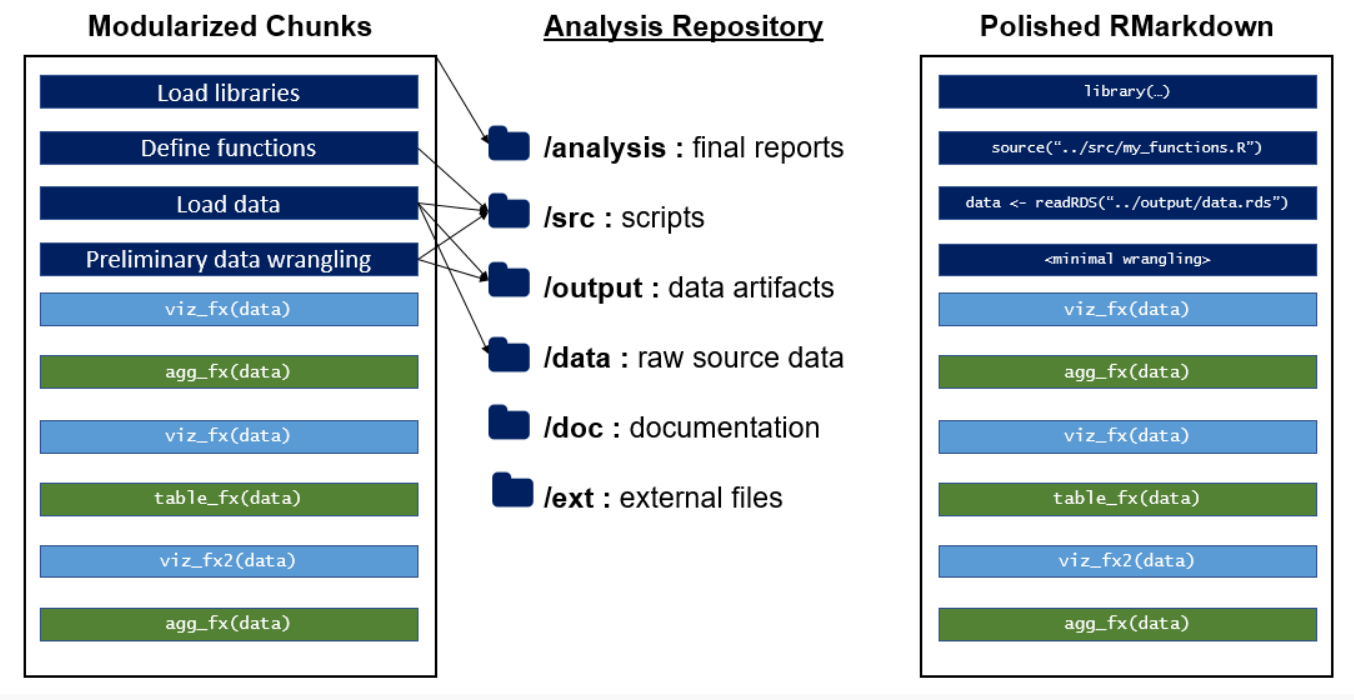
\includegraphics{../external/images/setup_4_markdown_project.PNG}

\url{https://emilyriederer.netlify.com/post/rmarkdown-driven-development/}

\end{frame}

\begin{frame}

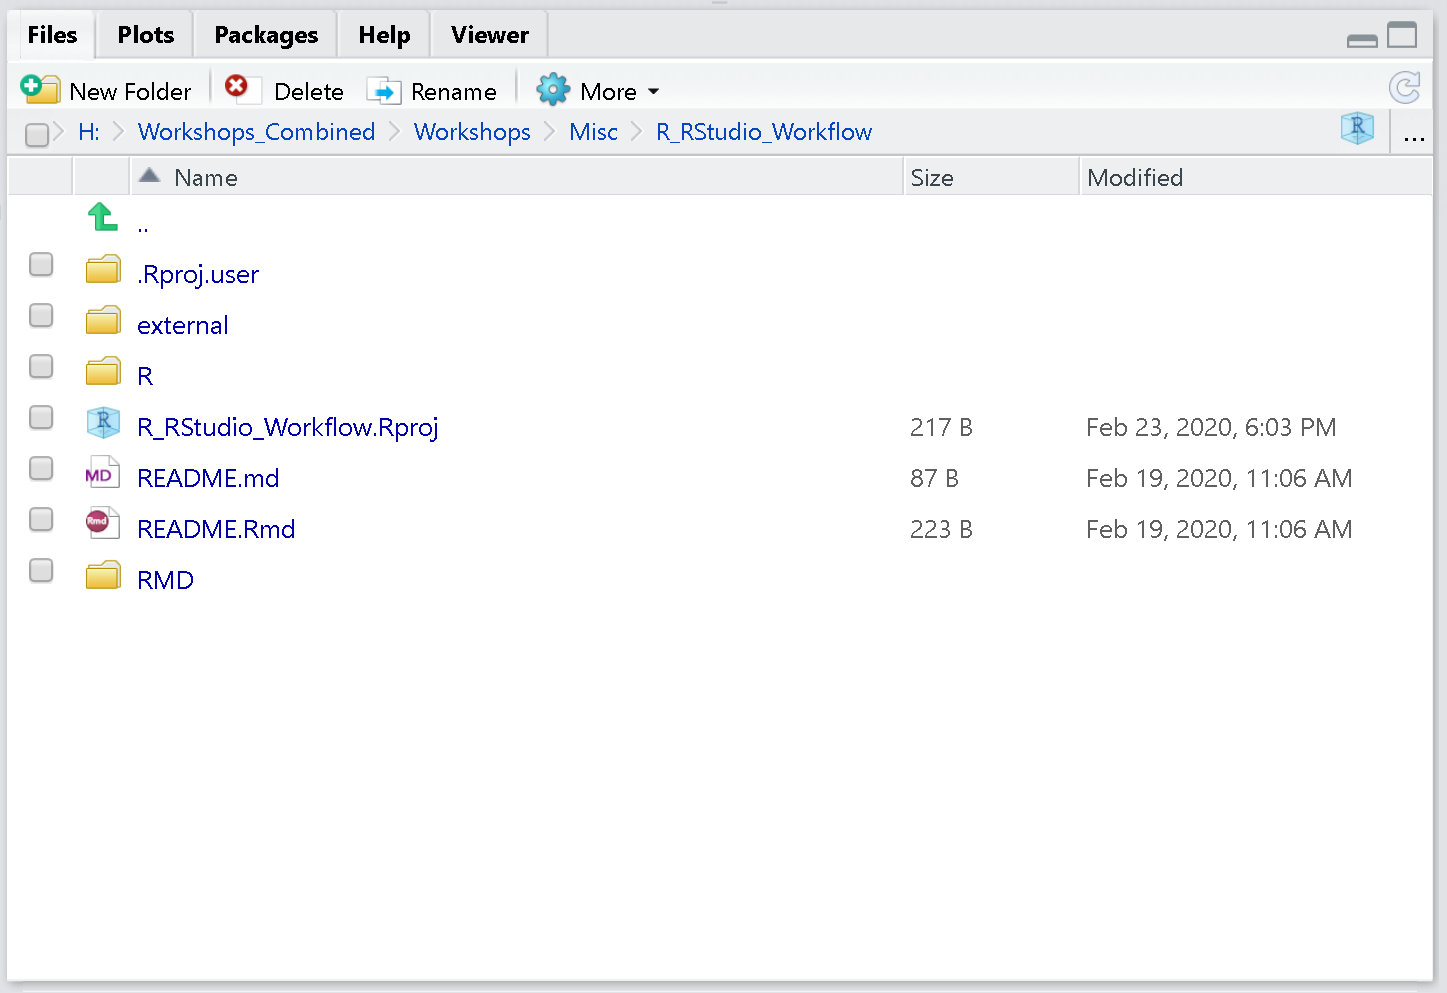
\includegraphics{../external/images/this_project.PNG}

\end{frame}

\begin{frame}{Organize your project folders and markdown}
\protect\hypertarget{organize-your-project-folders-and-markdown}{}

\begin{itemize}[<+->]
\tightlist
\item
  What works for you?
\item
  What works for your organization or team?
\item
  Maximize utility, minimize complexity
\end{itemize}

\end{frame}

\hypertarget{part-1}{%
\section{Part 1}\label{part-1}}

\hypertarget{part-2-rstudio-project-setup}{%
\section{Part 2: RStudio \& Project
setup}\label{part-2-rstudio-project-setup}}

\begin{frame}{RStudio}
\protect\hypertarget{rstudio}{}

\begin{itemize}[<+->]
\tightlist
\item
  IDE: Integrated development environment
\item
  RStudio: Does so much

  \begin{itemize}[<+->]
  \tightlist
  \item
    We scratch the surface here
  \end{itemize}
\item
  Quick walk through

  \begin{itemize}[<+->]
  \tightlist
  \item
    Followed by specific set up
  \item
    Generally, but
  \item
    Also for this workshop
  \end{itemize}
\end{itemize}

\end{frame}

\begin{frame}{RStudio Setup}
\protect\hypertarget{rstudio-setup}{}

\begin{itemize}[<+->]
\tightlist
\item
  Download R and Rstudio

  \begin{itemize}[<+->]
  \tightlist
  \item
    Strongly recommend Microsoft R
    (\url{https://mran.microsoft.com/open})
  \item
    Comes with Intel MKL
  \end{itemize}
\item
  Plain R is fine (\url{https://cran.r-project.org/})

  \begin{itemize}[<+->]
  \tightlist
  \item
    Can relink to faster libraries
  \end{itemize}
\item
  Download RStudio (\url{https://www.rstudio.com/})
\end{itemize}

\end{frame}

\begin{frame}{RStudio Environment}
\protect\hypertarget{rstudio-environment}{}

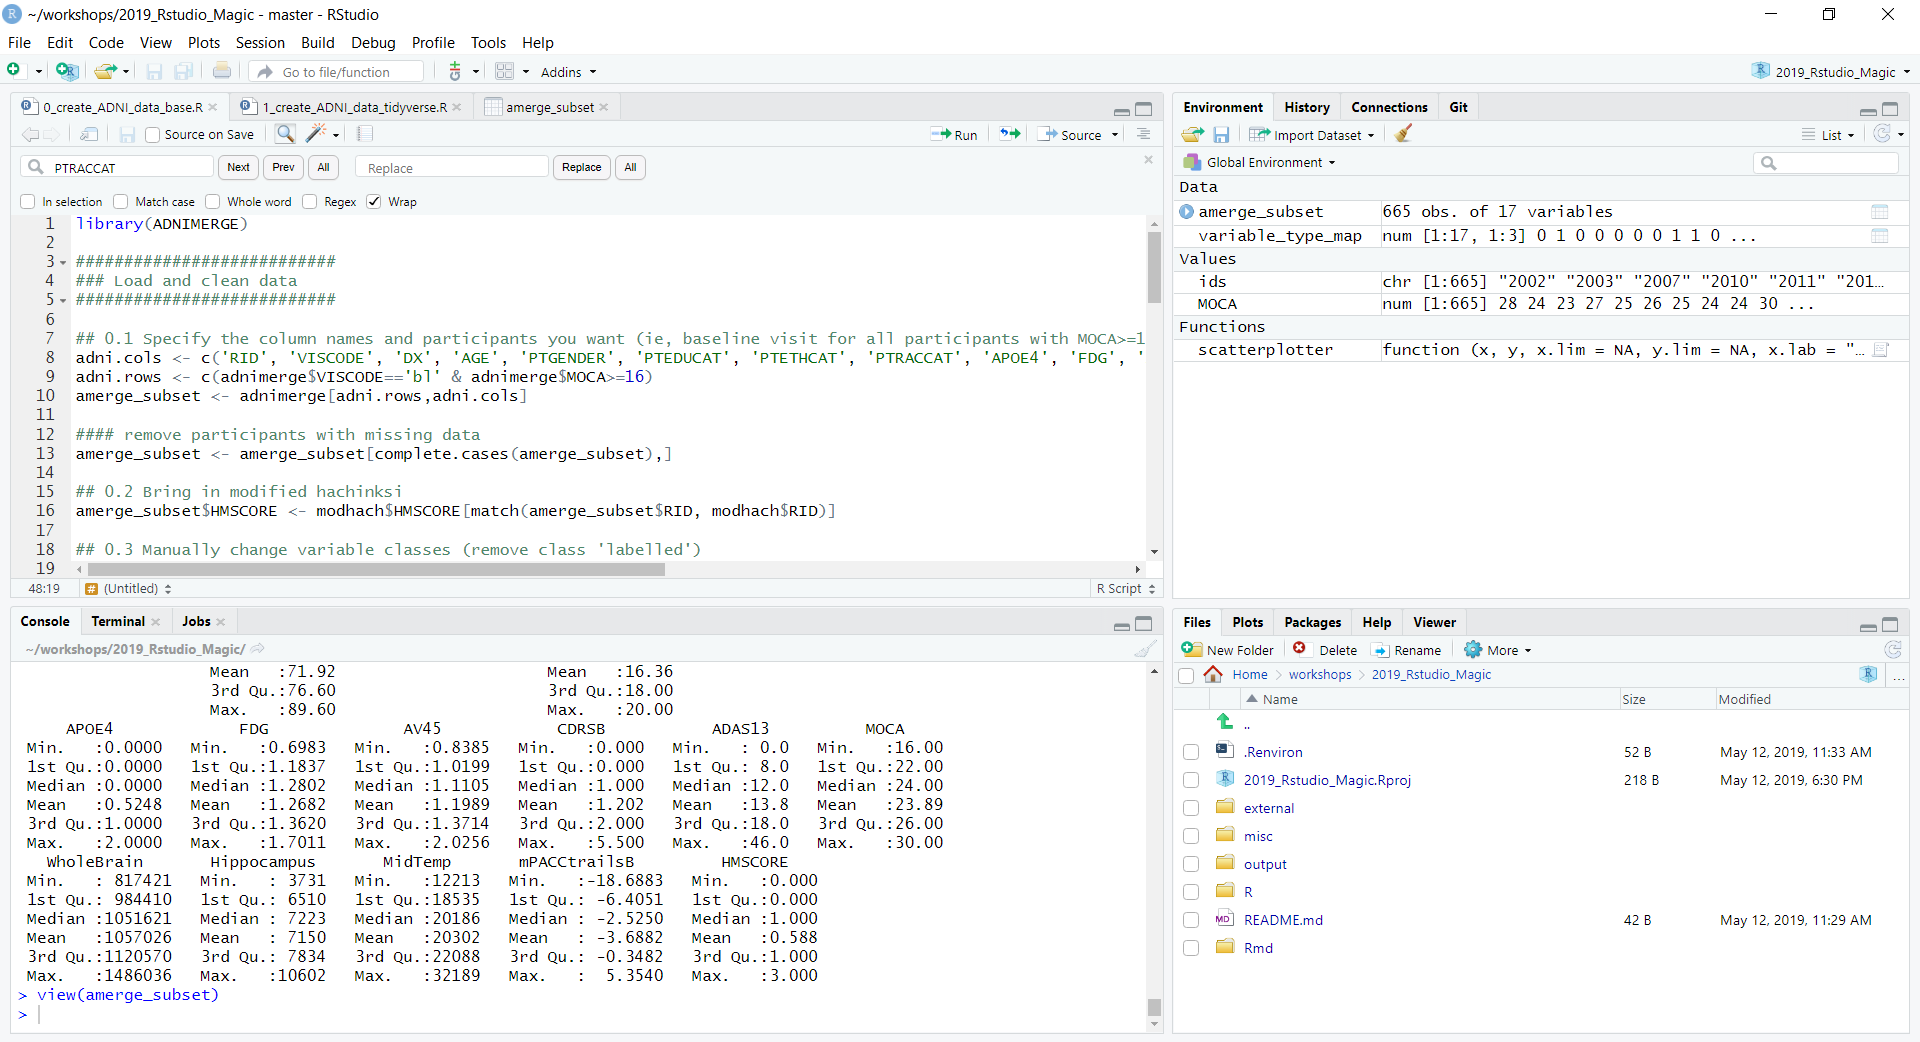
\includegraphics{../external/images/rstudio_terminal_0.PNG}

\end{frame}

\begin{frame}

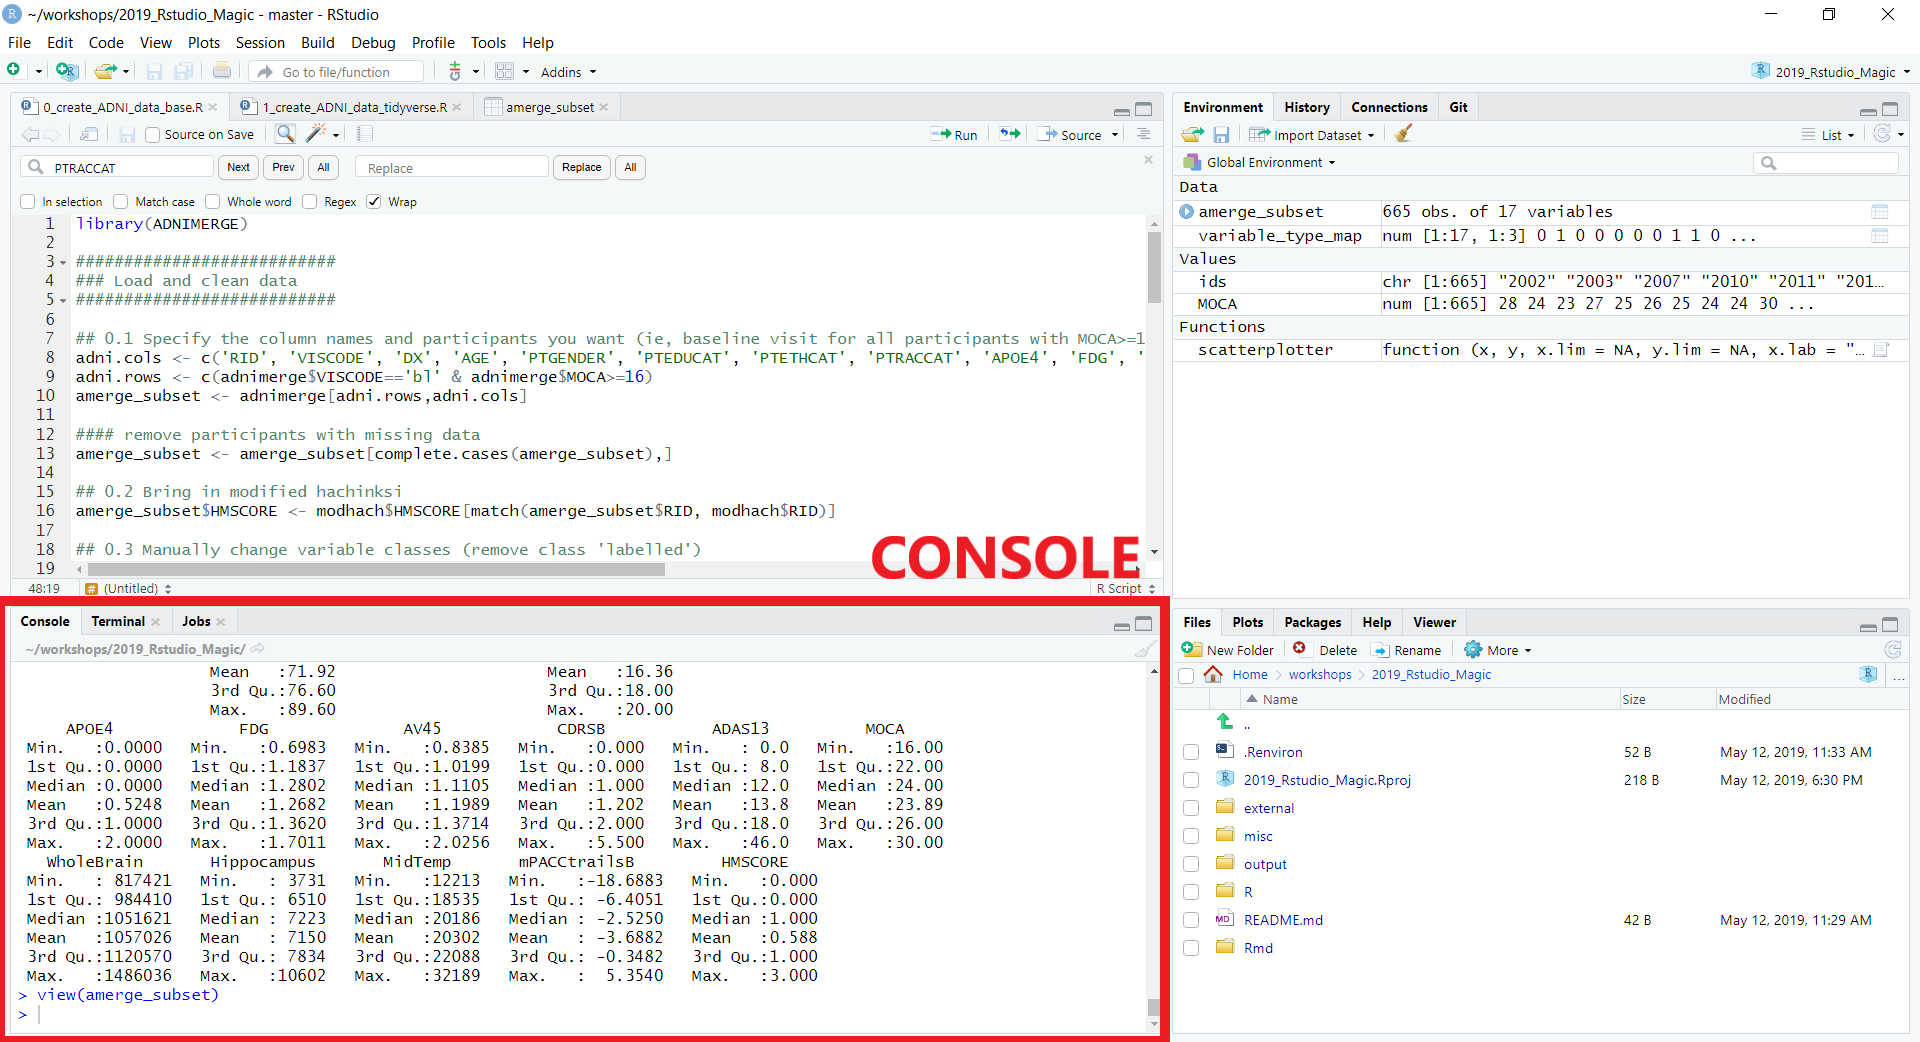
\includegraphics{../external/images/rstudio_terminal_1_CONSOLE.png}

\end{frame}

\begin{frame}

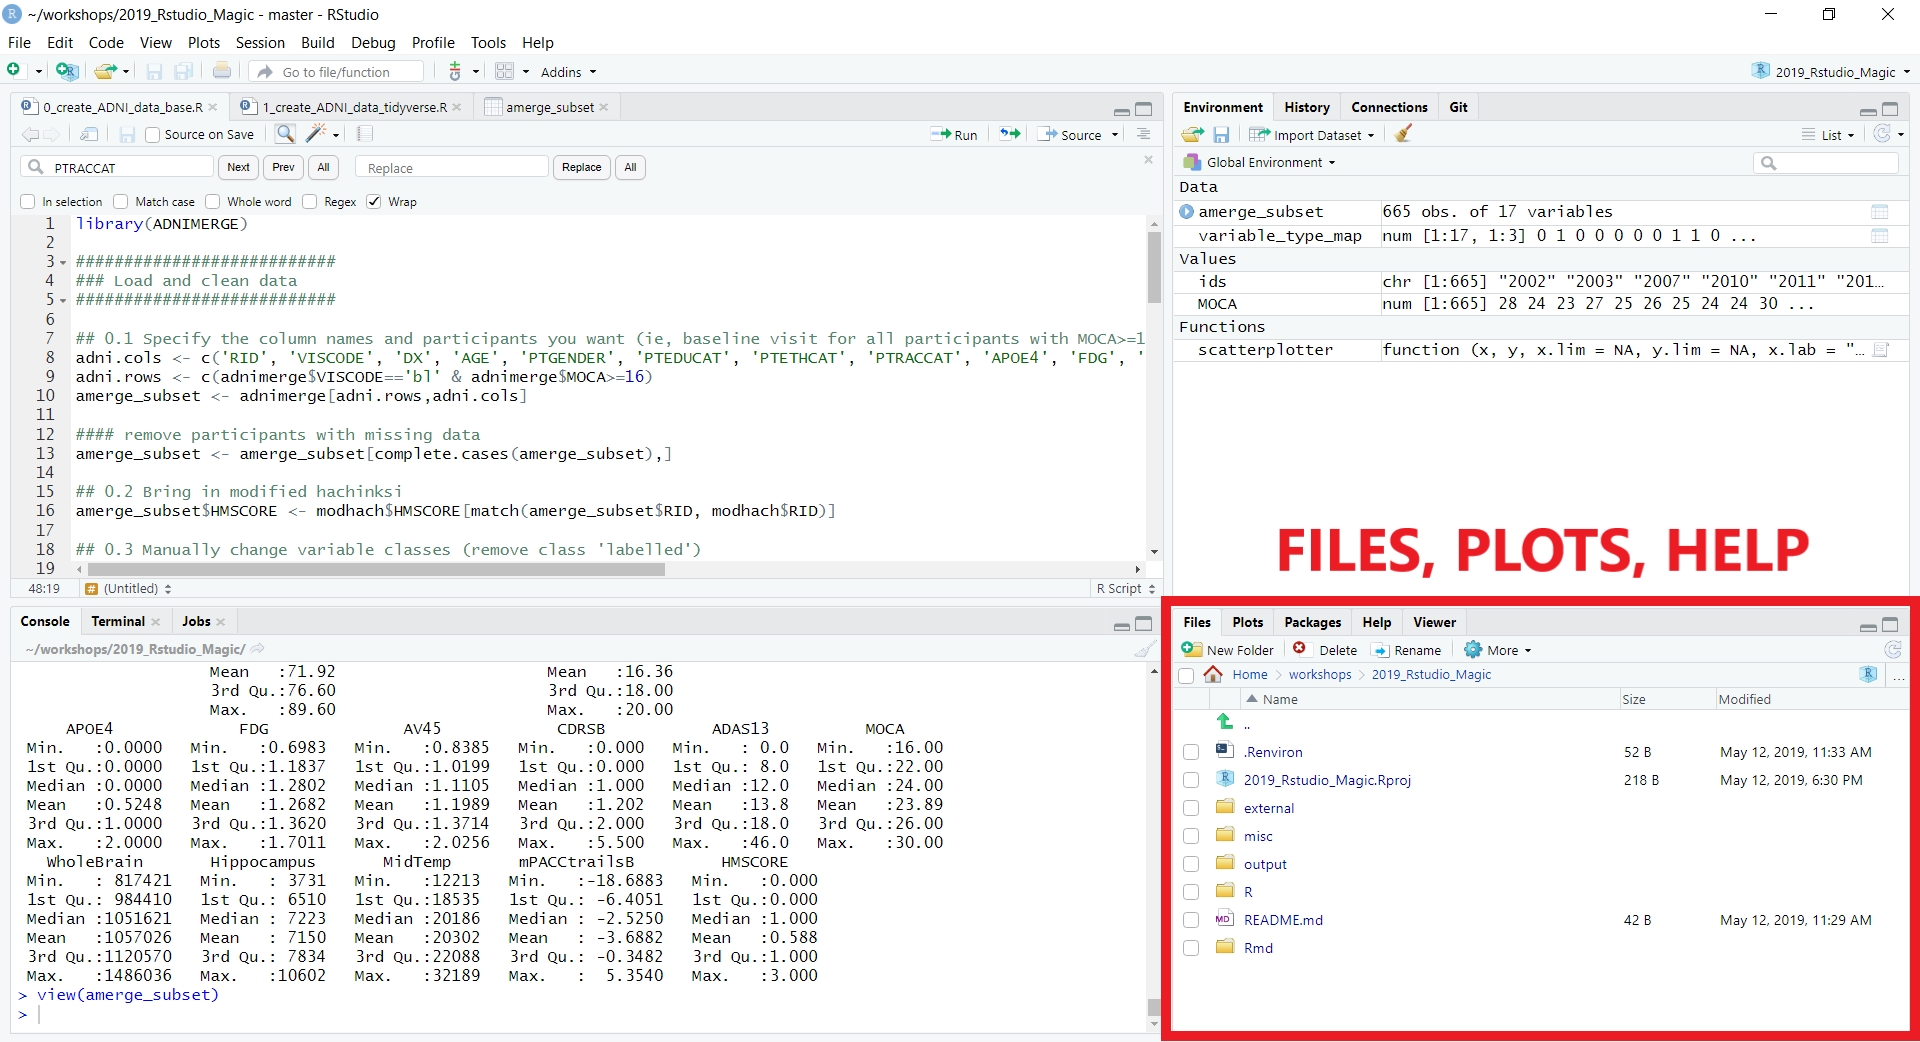
\includegraphics{../external/images/rstudio_terminal_2_FILES.png}

\end{frame}

\begin{frame}

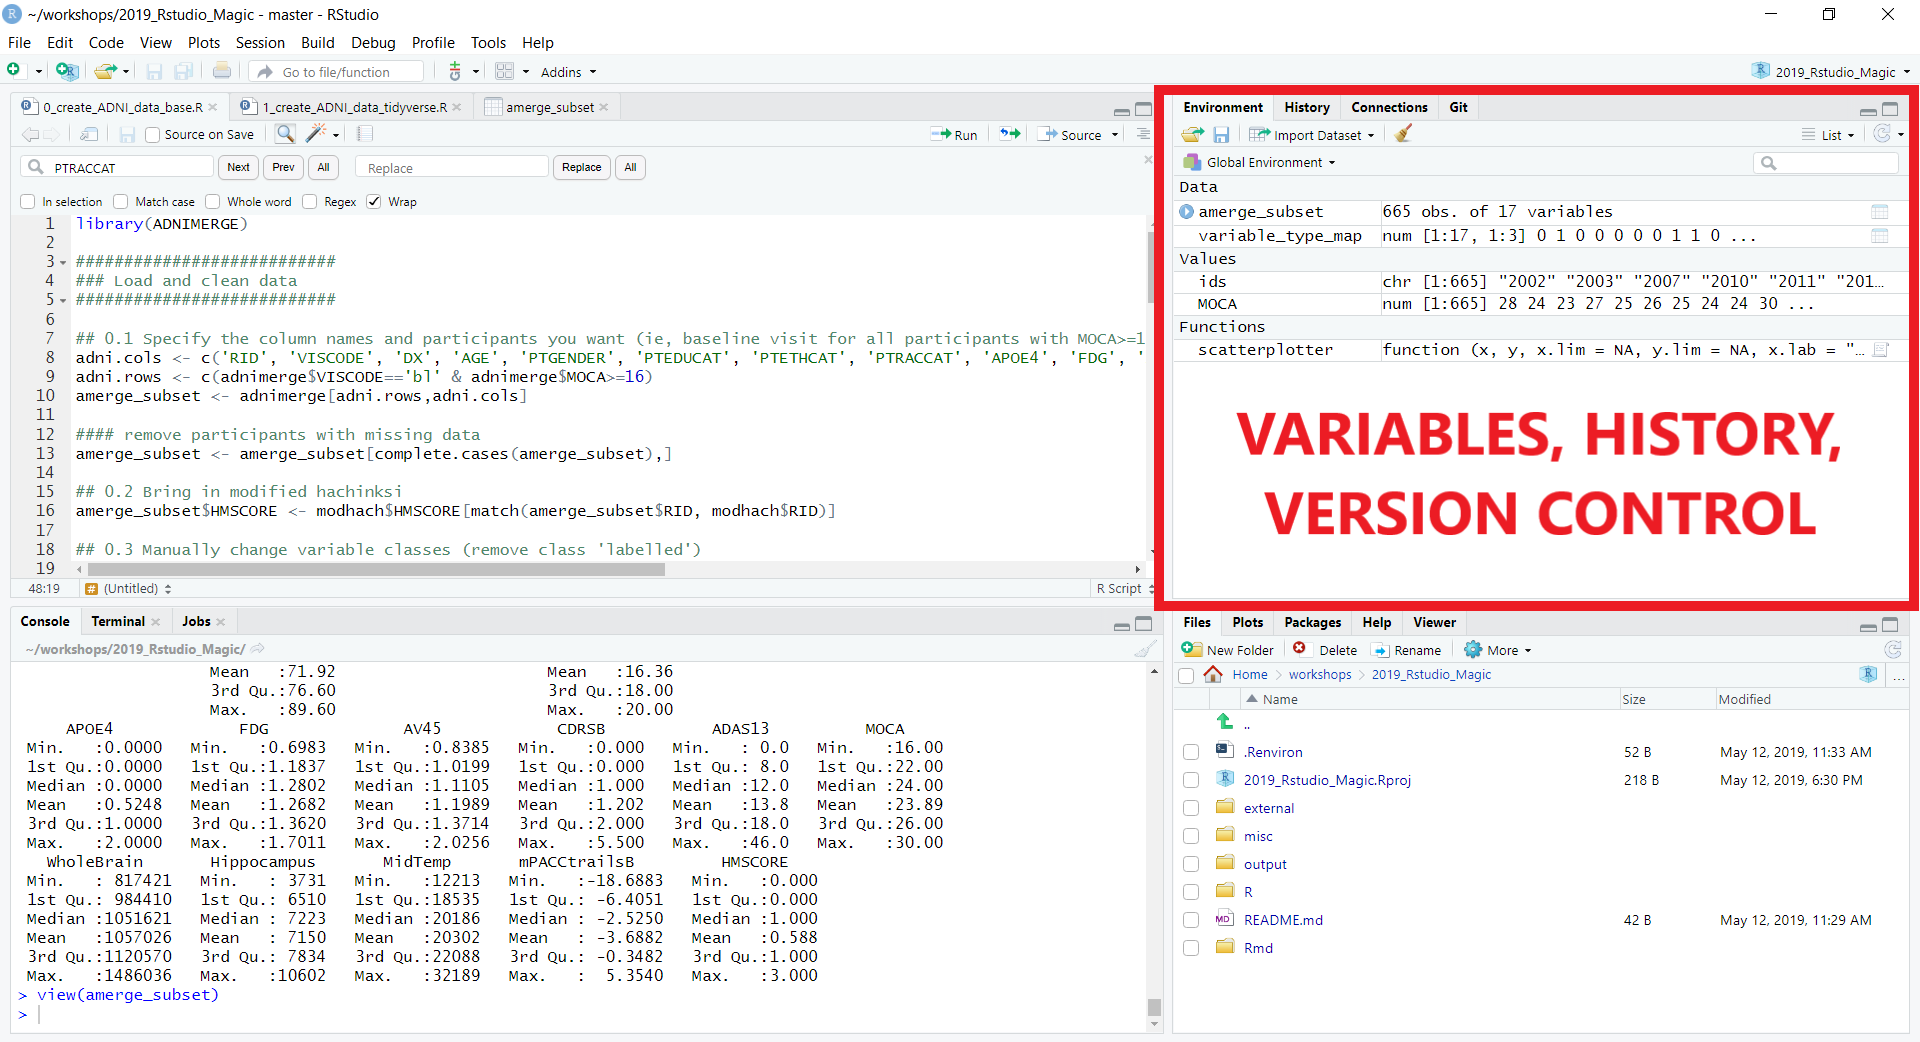
\includegraphics{../external/images/rstudio_terminal_3_ENV.png}

\end{frame}

\begin{frame}

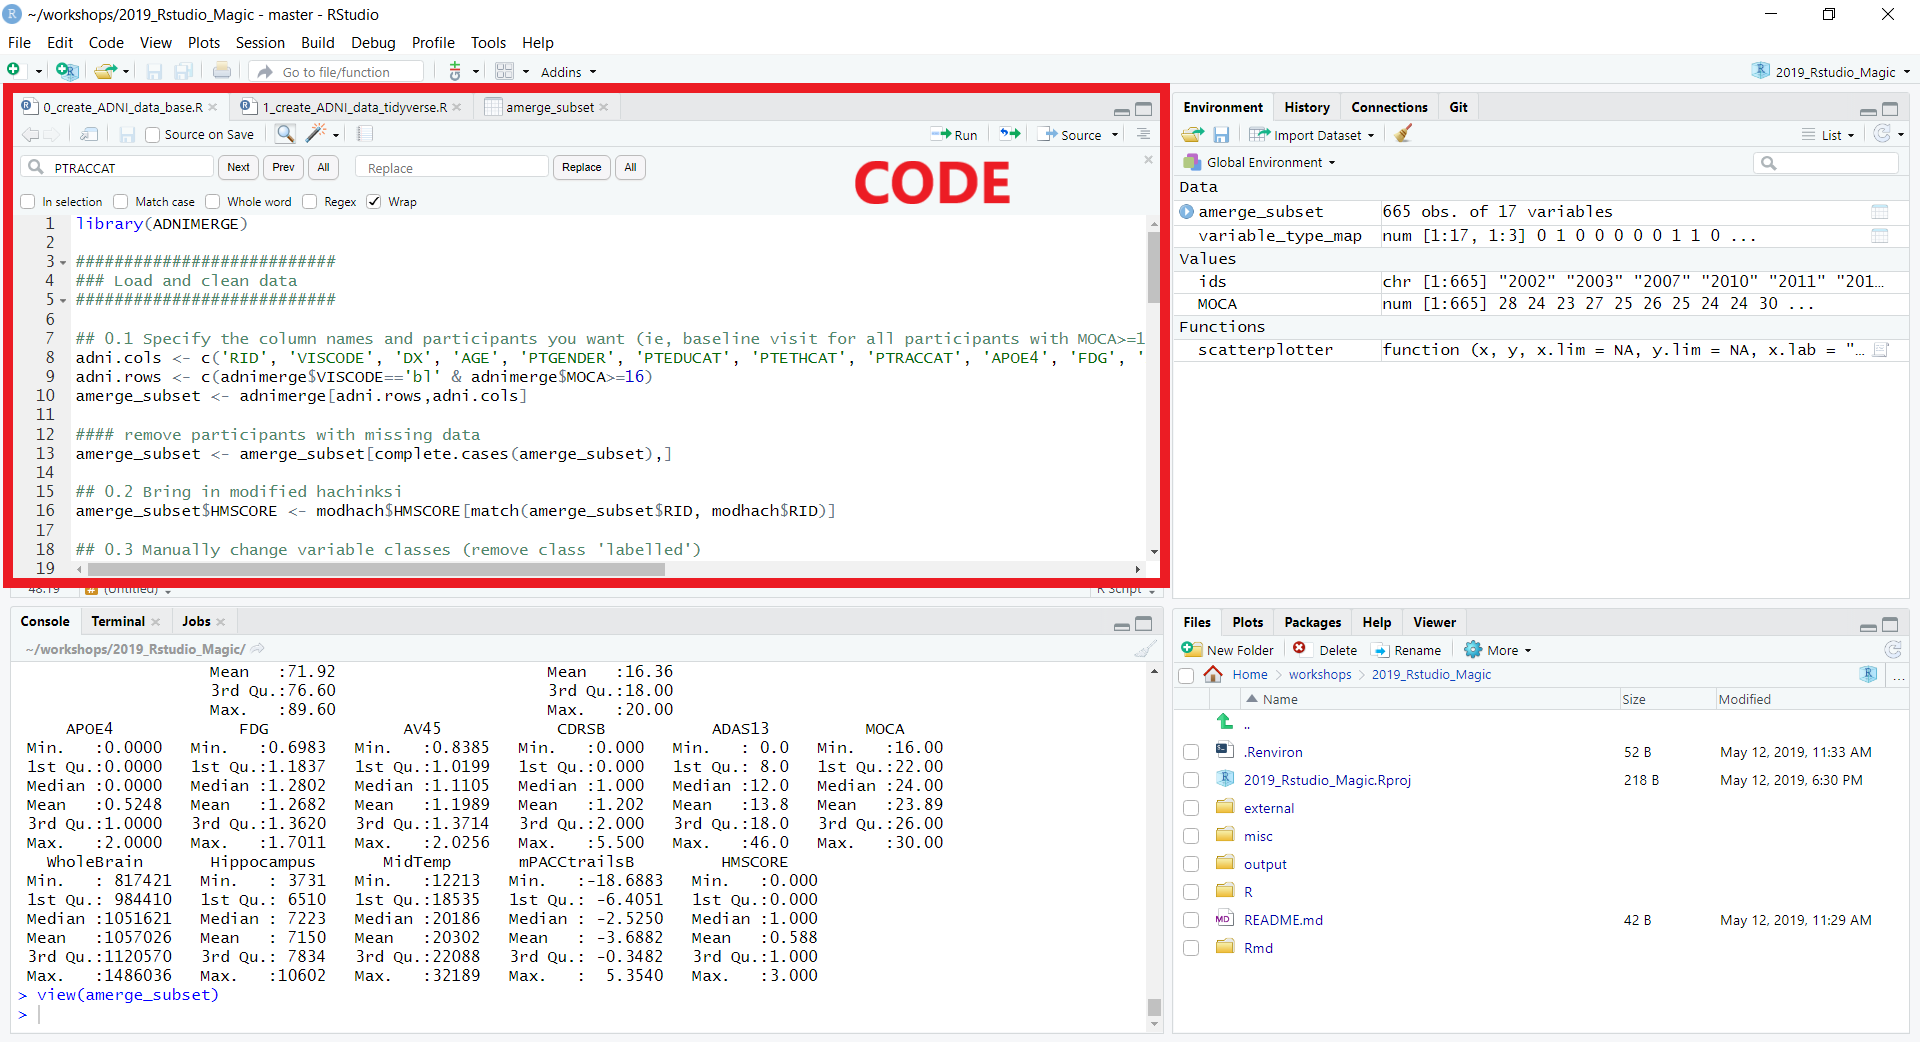
\includegraphics{../external/images/rstudio_terminal_4_CODE.png}

\end{frame}

\begin{frame}

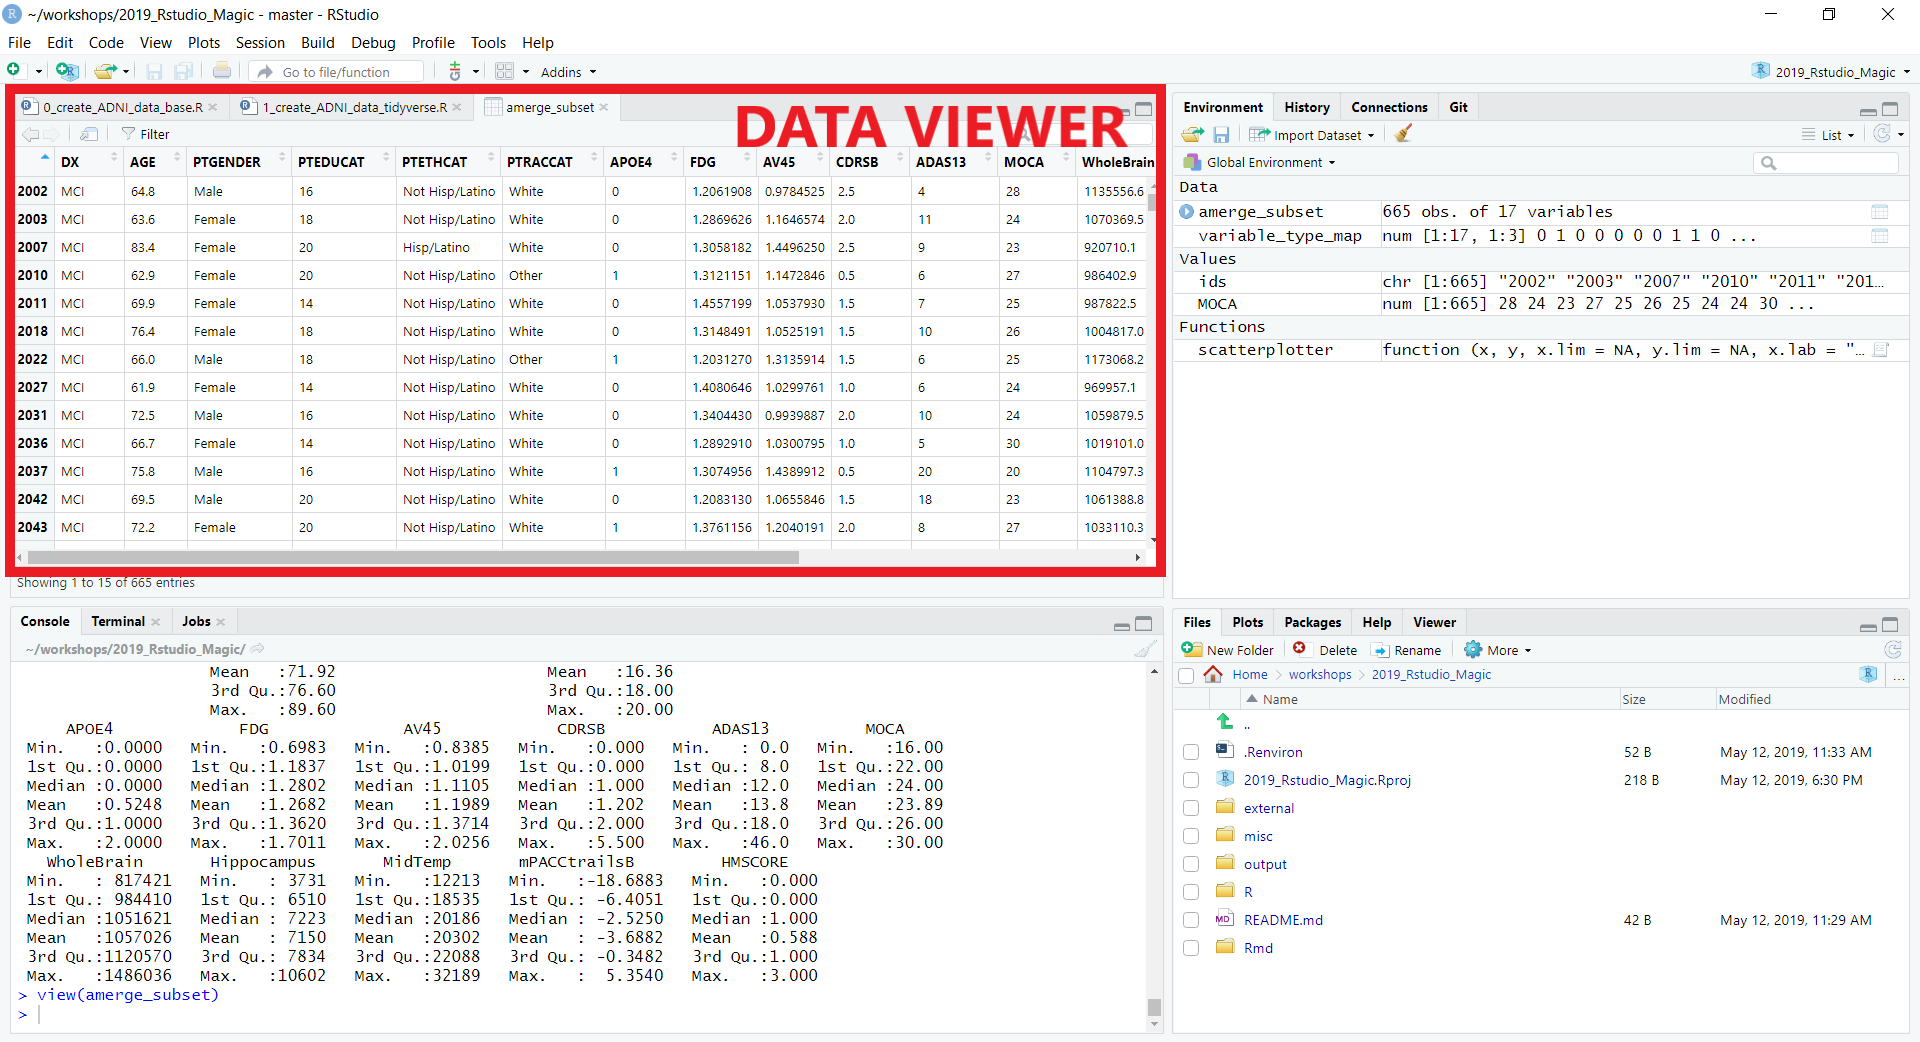
\includegraphics{../external/images/rstudio_terminal_5_DATA.png}

\end{frame}

\begin{frame}{Benefits of RStudio}
\protect\hypertarget{benefits-of-rstudio}{}

\begin{itemize}[<+->]
\tightlist
\item
  Built-in integration with version control (git or SVN)
\item
  R Markdown

  \begin{itemize}[<+->]
  \tightlist
  \item
    Save and execute code
  \item
    Generate high quality reports that can be shared
  \item
    Create presentations (like this one!)
  \item
    Even write papers
  \item
    This workshop

    \begin{itemize}[<+->]
    \tightlist
    \item
      See
      \url{https://github.com/derekbeaton/Workshops/tree/master/Misc/R_RStudio_Workflow}
    \end{itemize}
  \end{itemize}
\item
  Python, D3 (JavaScript), SQL, Shiny, LaTeX, Git/SVN, HTML/CSS, and so
  much more.
\end{itemize}

\end{frame}

\begin{frame}{RStudio is more}
\protect\hypertarget{rstudio-is-more}{}

\begin{itemize}[<+->]
\tightlist
\item
  Not just an IDE (integrated development environment)
\item
  A company
\item
  A community
\item
  A conference
\item
  A centralized resource
\end{itemize}

\end{frame}

\begin{frame}{RStudio Resources}
\protect\hypertarget{rstudio-resources}{}

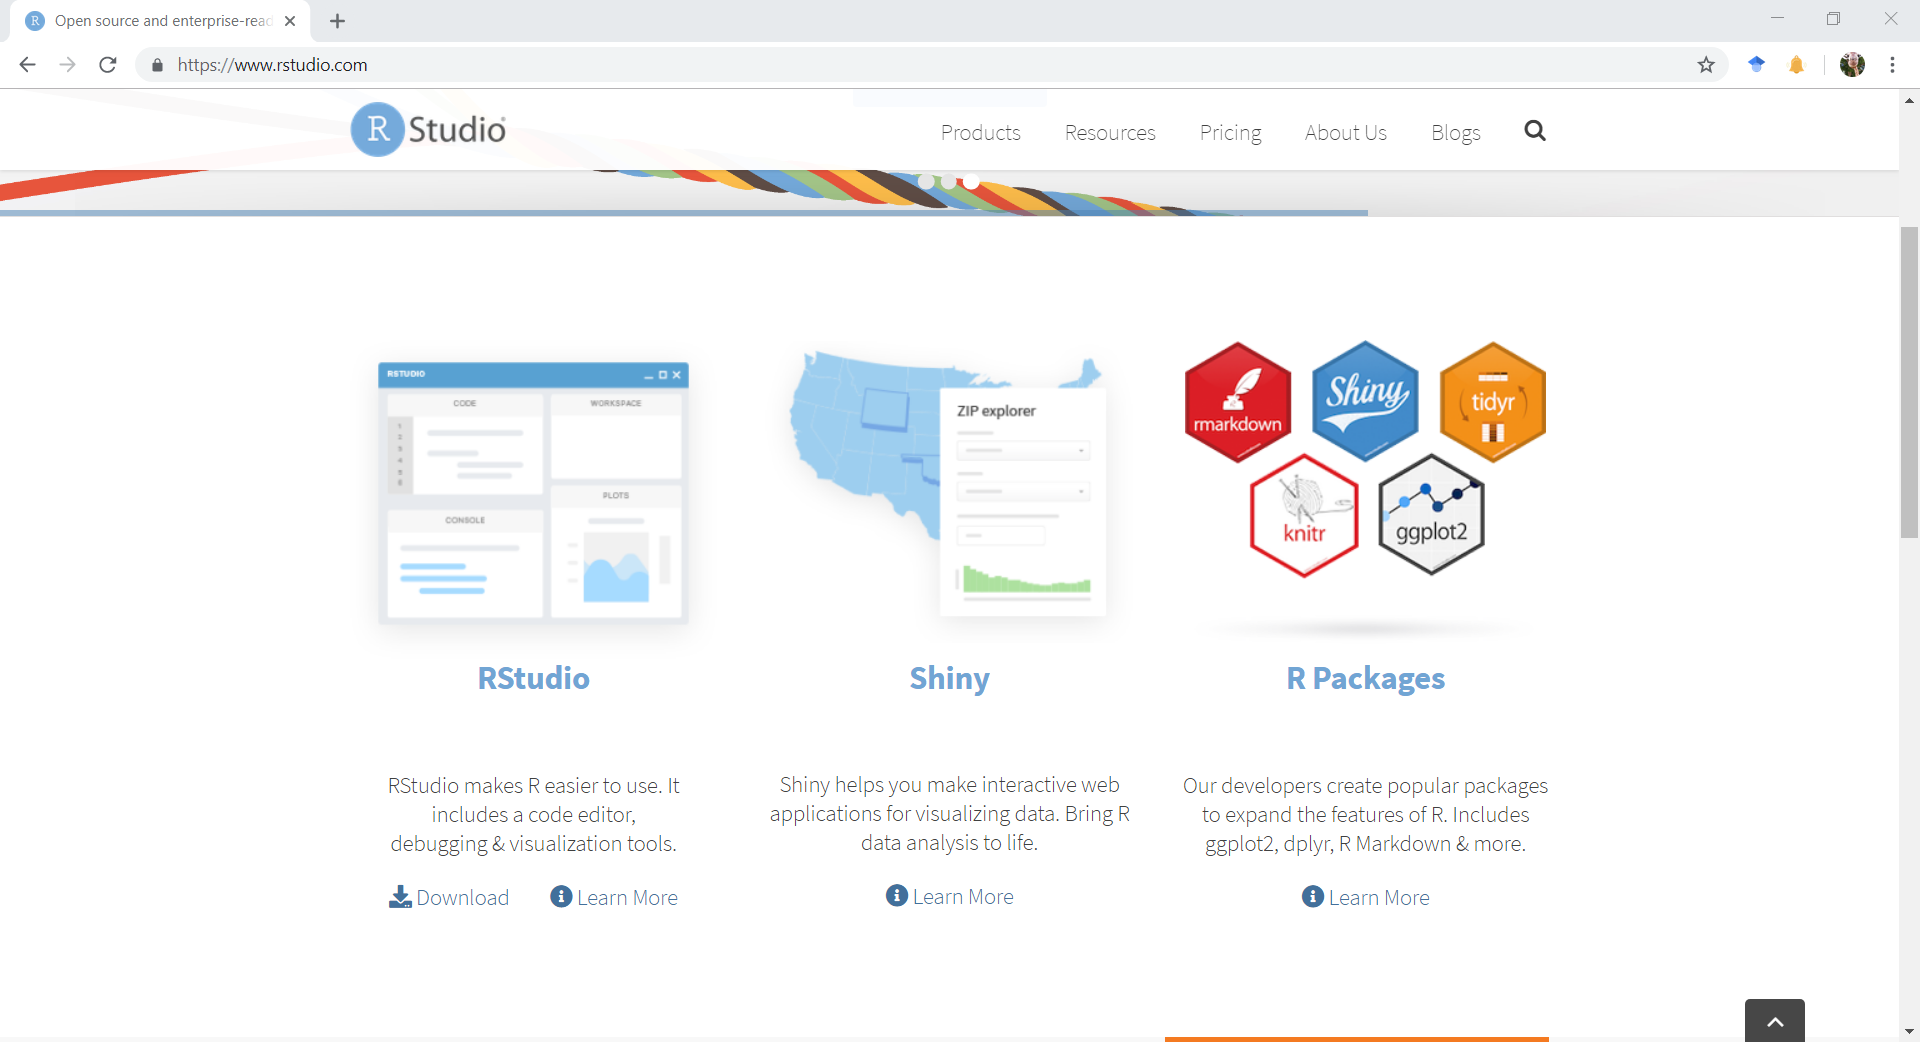
\includegraphics{../external/images/rstudio_dot_com_1_main.PNG}

\end{frame}

\begin{frame}

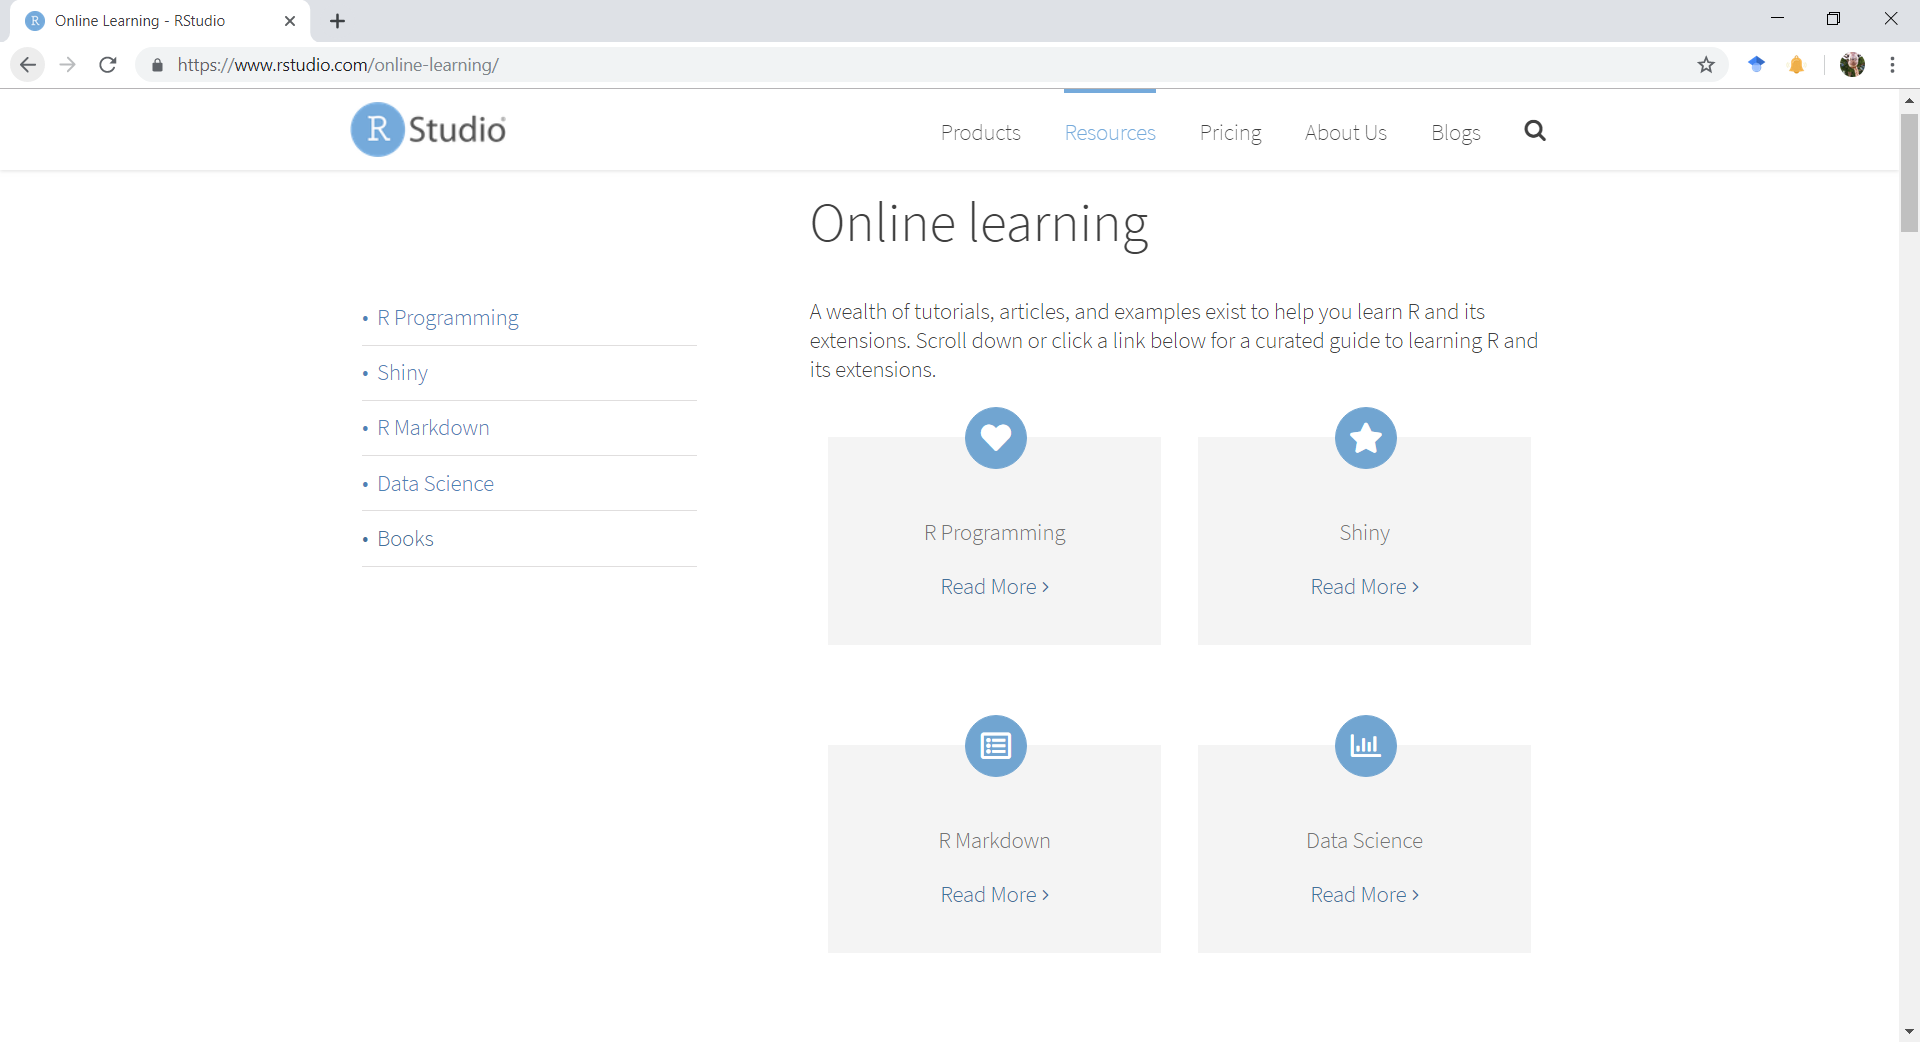
\includegraphics{../external/images/rstudio_dot_com_2_learning.PNG}

\end{frame}

\begin{frame}

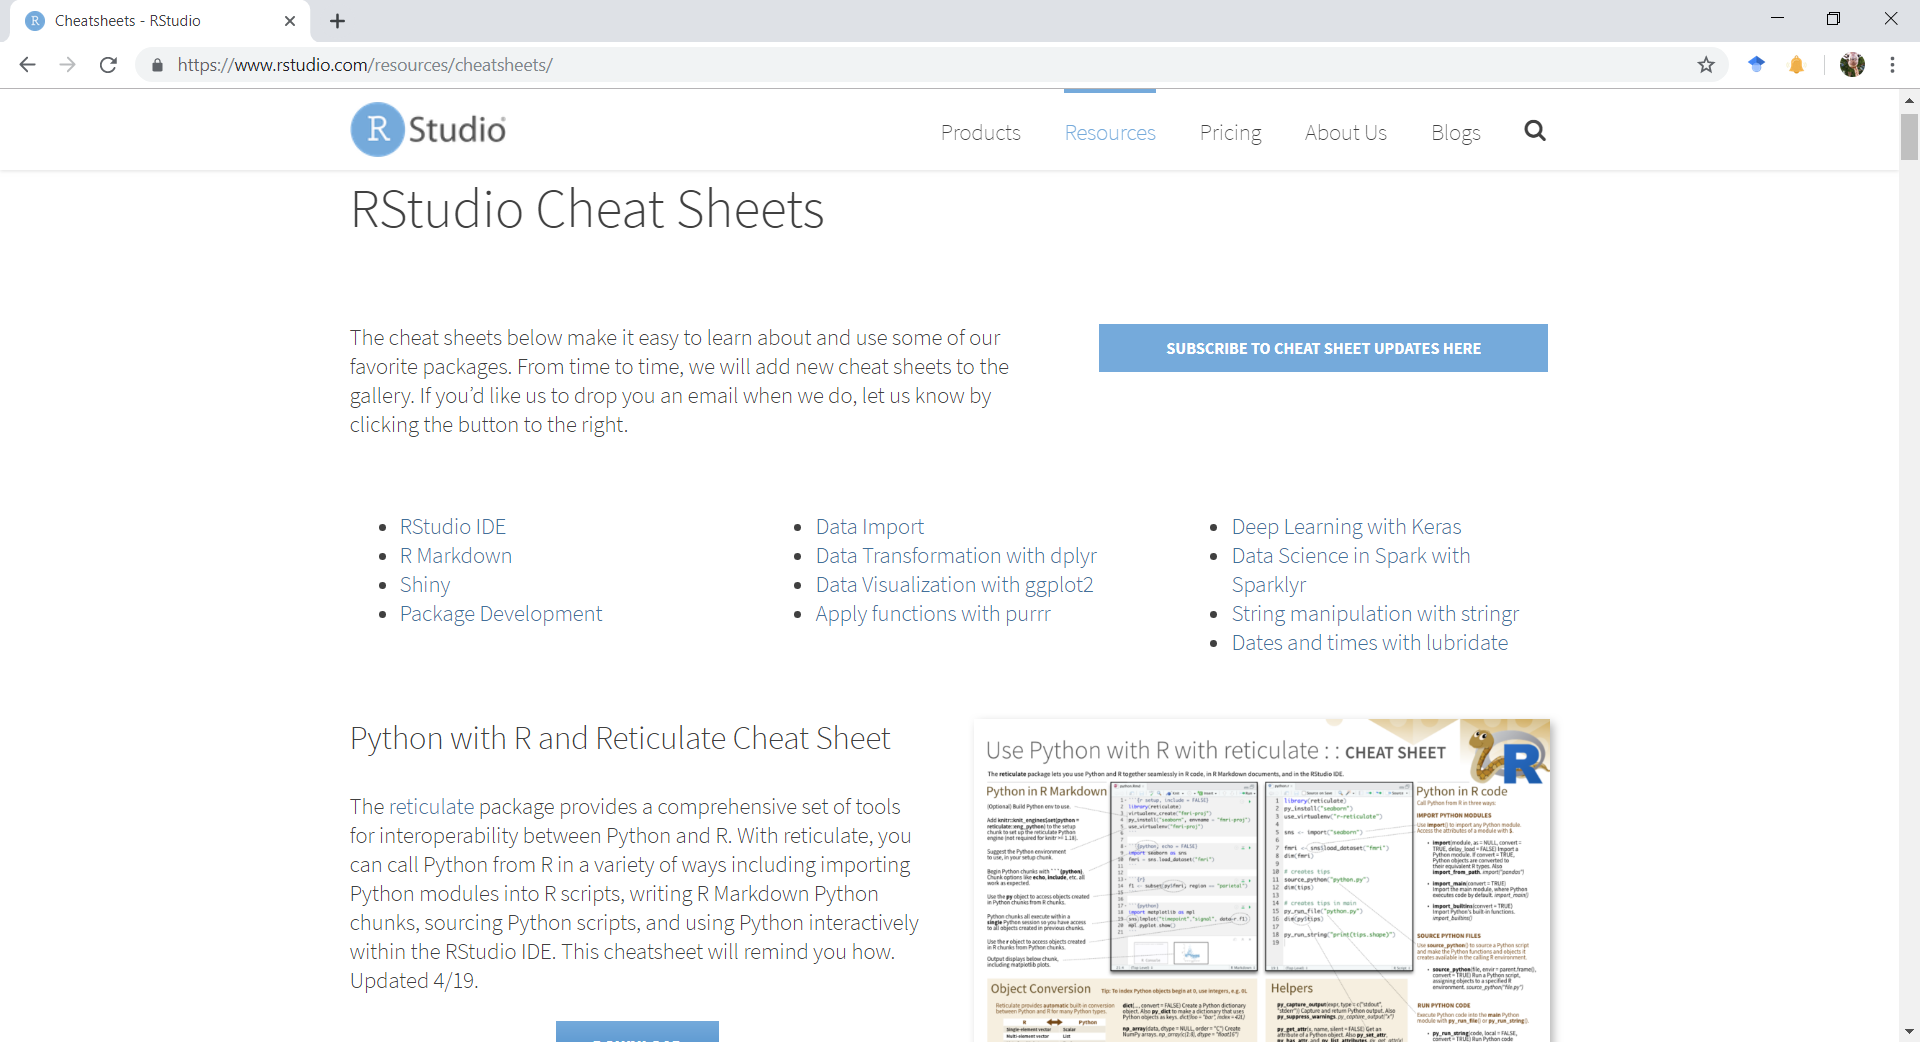
\includegraphics{../external/images/rstudio_dot_com_3_cheats.PNG}

\end{frame}

\hypertarget{project-and-environment-setup}{%
\subsection{Project and Environment
Setup}\label{project-and-environment-setup}}

\begin{frame}{RStudio Setup}
\protect\hypertarget{rstudio-setup-1}{}

\begin{itemize}[<+->]
\tightlist
\item
  See \url{https://jennybc.github.io/2014-05-12-ubc/r-setup.html} for a
  detailed guide
\end{itemize}

\end{frame}

\begin{frame}{For safety \& collaboration}
\protect\hypertarget{for-safety-collaboration}{}

\begin{itemize}[<+->]
\tightlist
\item
  RStudio projects

  \begin{itemize}[<+->]
  \tightlist
  \item
    ``RStudio projects make it straightforward to divide your work into
    multiple contexts, each with their own working directory, workspace,
    history, and source documents.''
  \item
    Allows for return to key states
  \end{itemize}
\item
  .Rproj files

  \begin{itemize}[<+->]
  \tightlist
  \item
    Basically a text file with some parameters for start up
    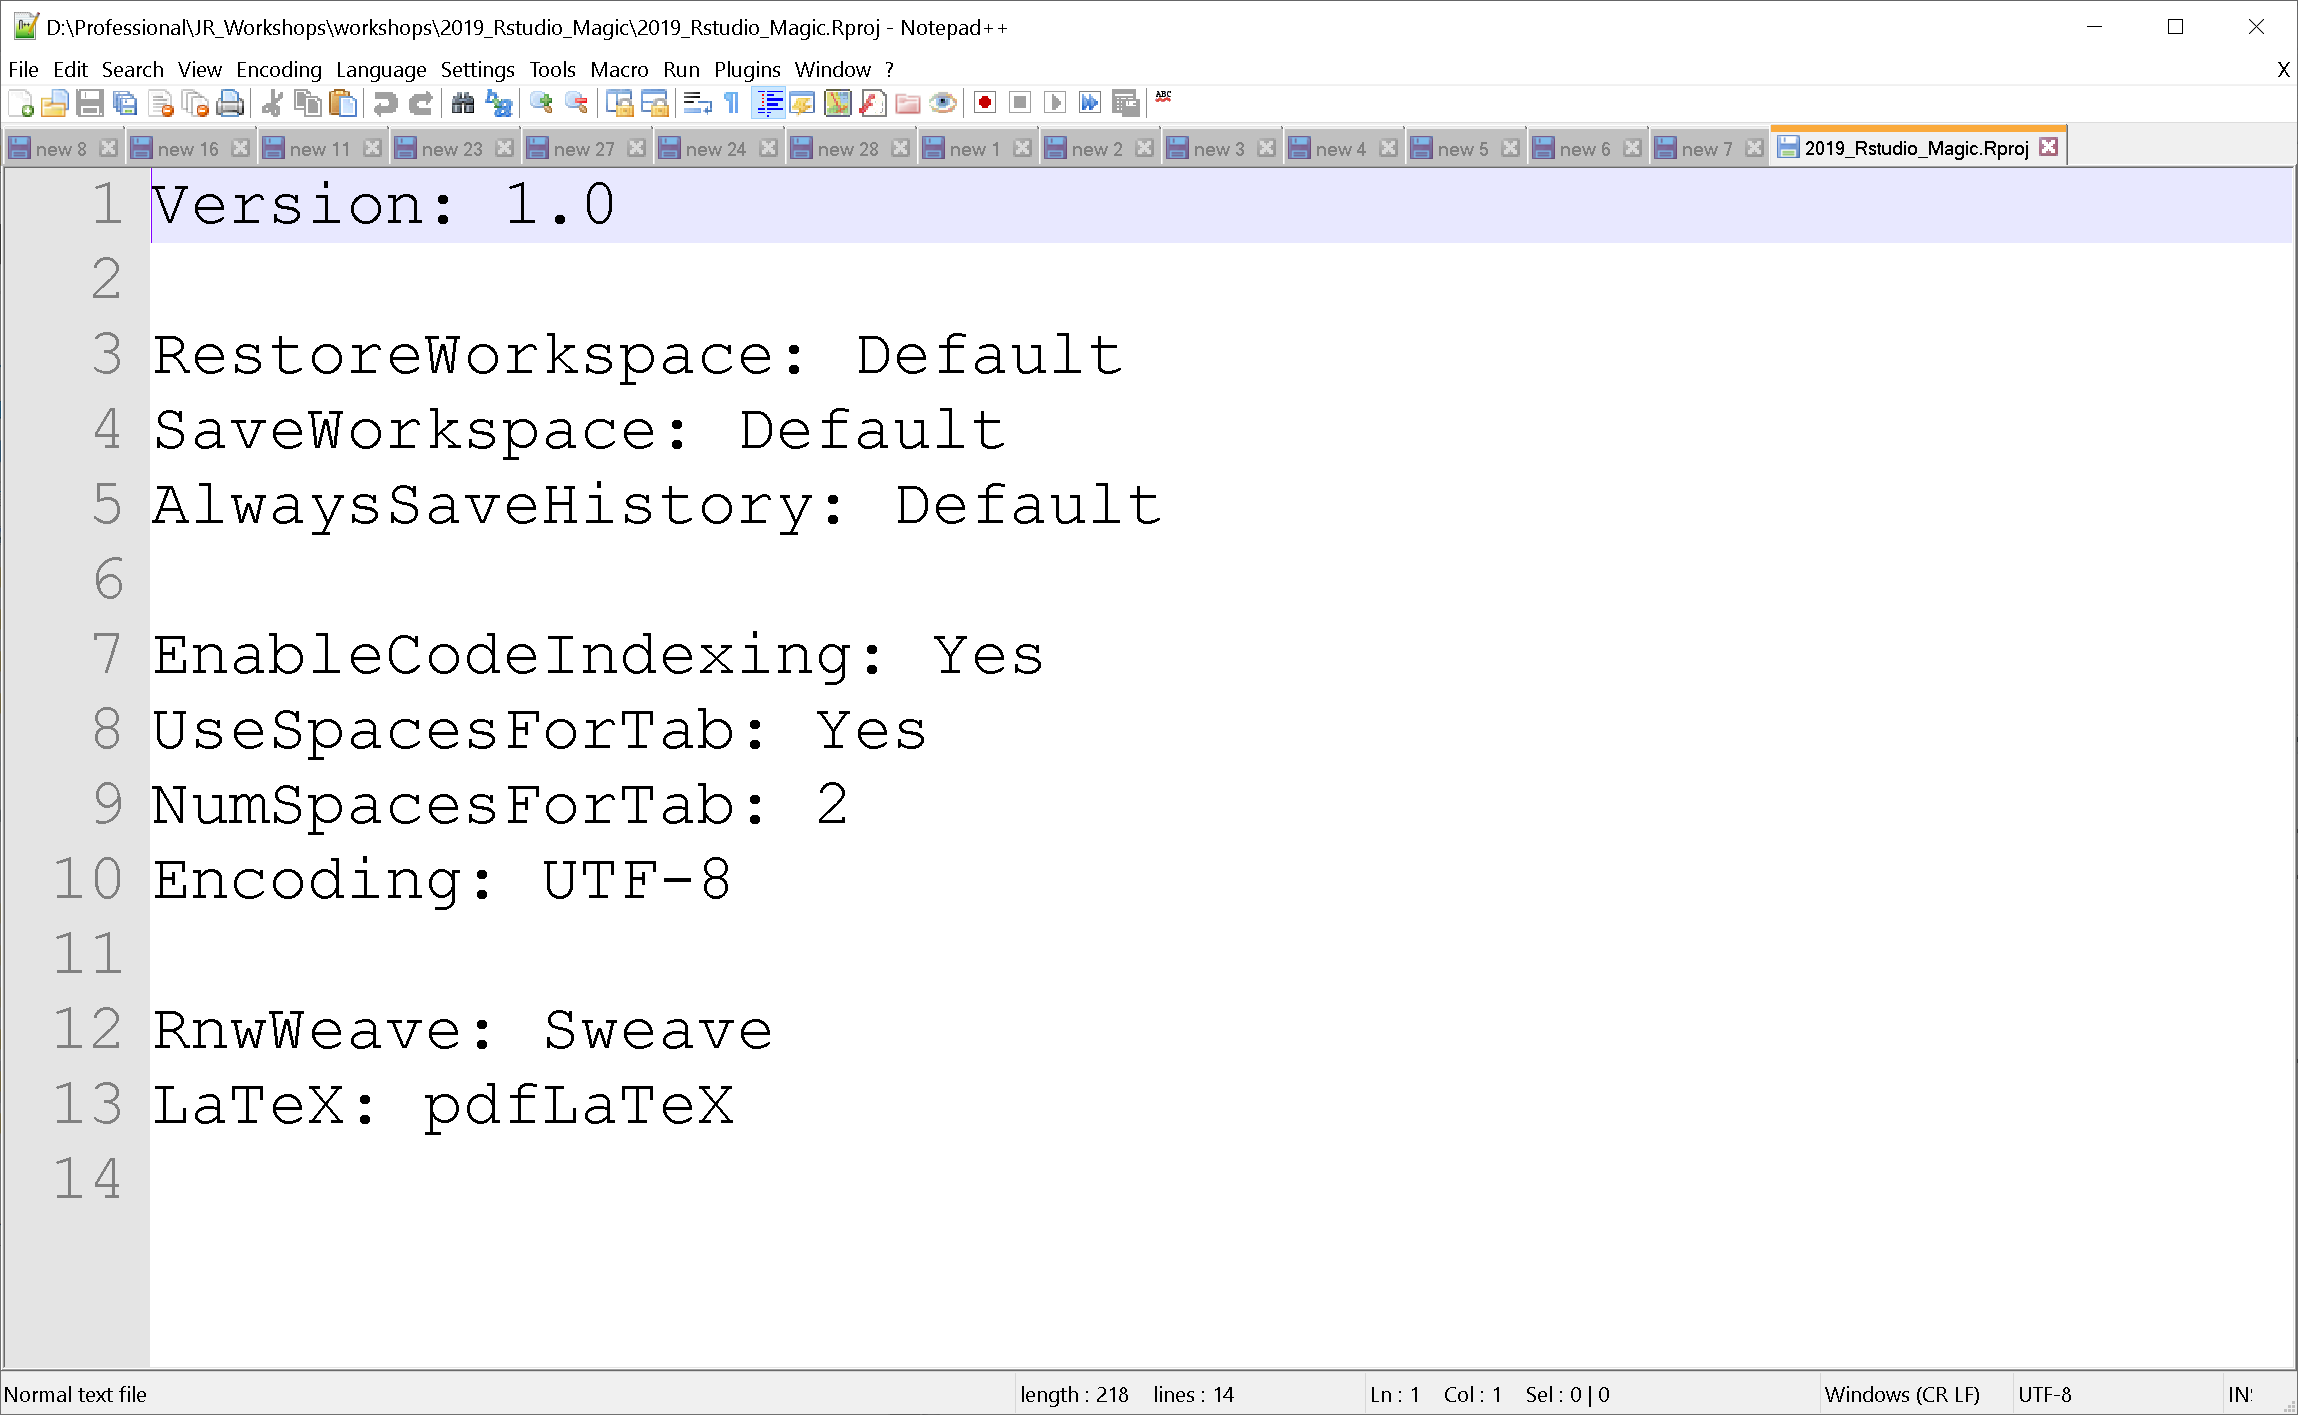
\includegraphics[width=0.5\textwidth,height=\textheight]{../external/images/Rproj_inside.PNG}
  \end{itemize}
\end{itemize}

\end{frame}

\begin{frame}{Projects}
\protect\hypertarget{projects}{}

Create a new one for:

\begin{itemize}[<+->]
\tightlist
\item
  a folder
\item
  packages
\item
  (and from) git repos:
  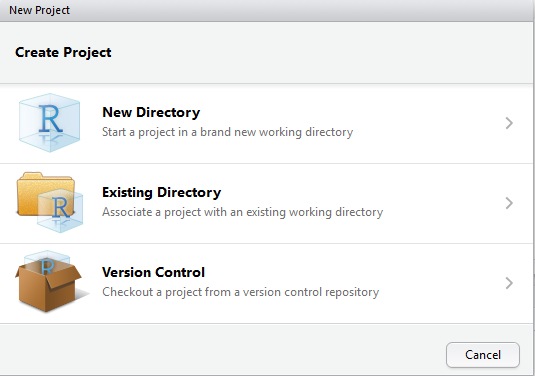
\includegraphics[width=0.75\textwidth,height=\textheight]{../external/images/setup_2_rstudio_project.PNG}
\end{itemize}

\end{frame}

\begin{frame}{What is Git?}
\protect\hypertarget{what-is-git}{}

SOMETHING

\end{frame}

\begin{frame}{Git \& Projects}
\protect\hypertarget{git-projects}{}

\begin{itemize}[<+->]
\tightlist
\item
  Git
\item
  Download git and link executable within RStudio
  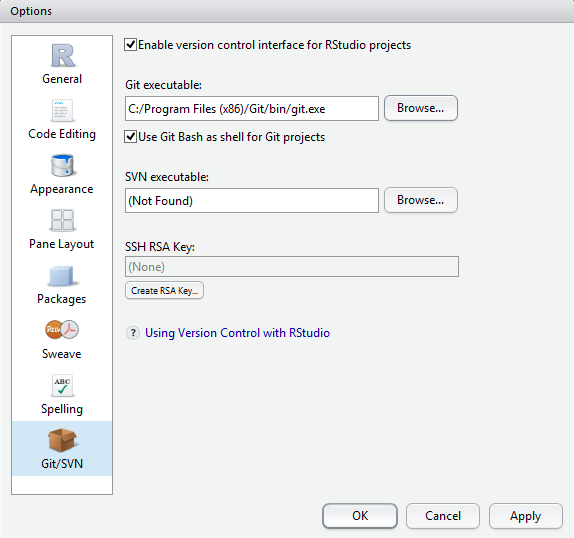
\includegraphics[width=0.6\textwidth,height=\textheight]{../external/images/setup_1_rstudio_git.PNG}
\end{itemize}

\end{frame}

\begin{frame}[fragile]{Format .gitignore}
\protect\hypertarget{format-.gitignore}{}

\begin{itemize}[<+->]
\tightlist
\item
  File types to ignore via version control
\item
  \texttt{**} before each extentions will match directories anywhere in
  the repo
\end{itemize}

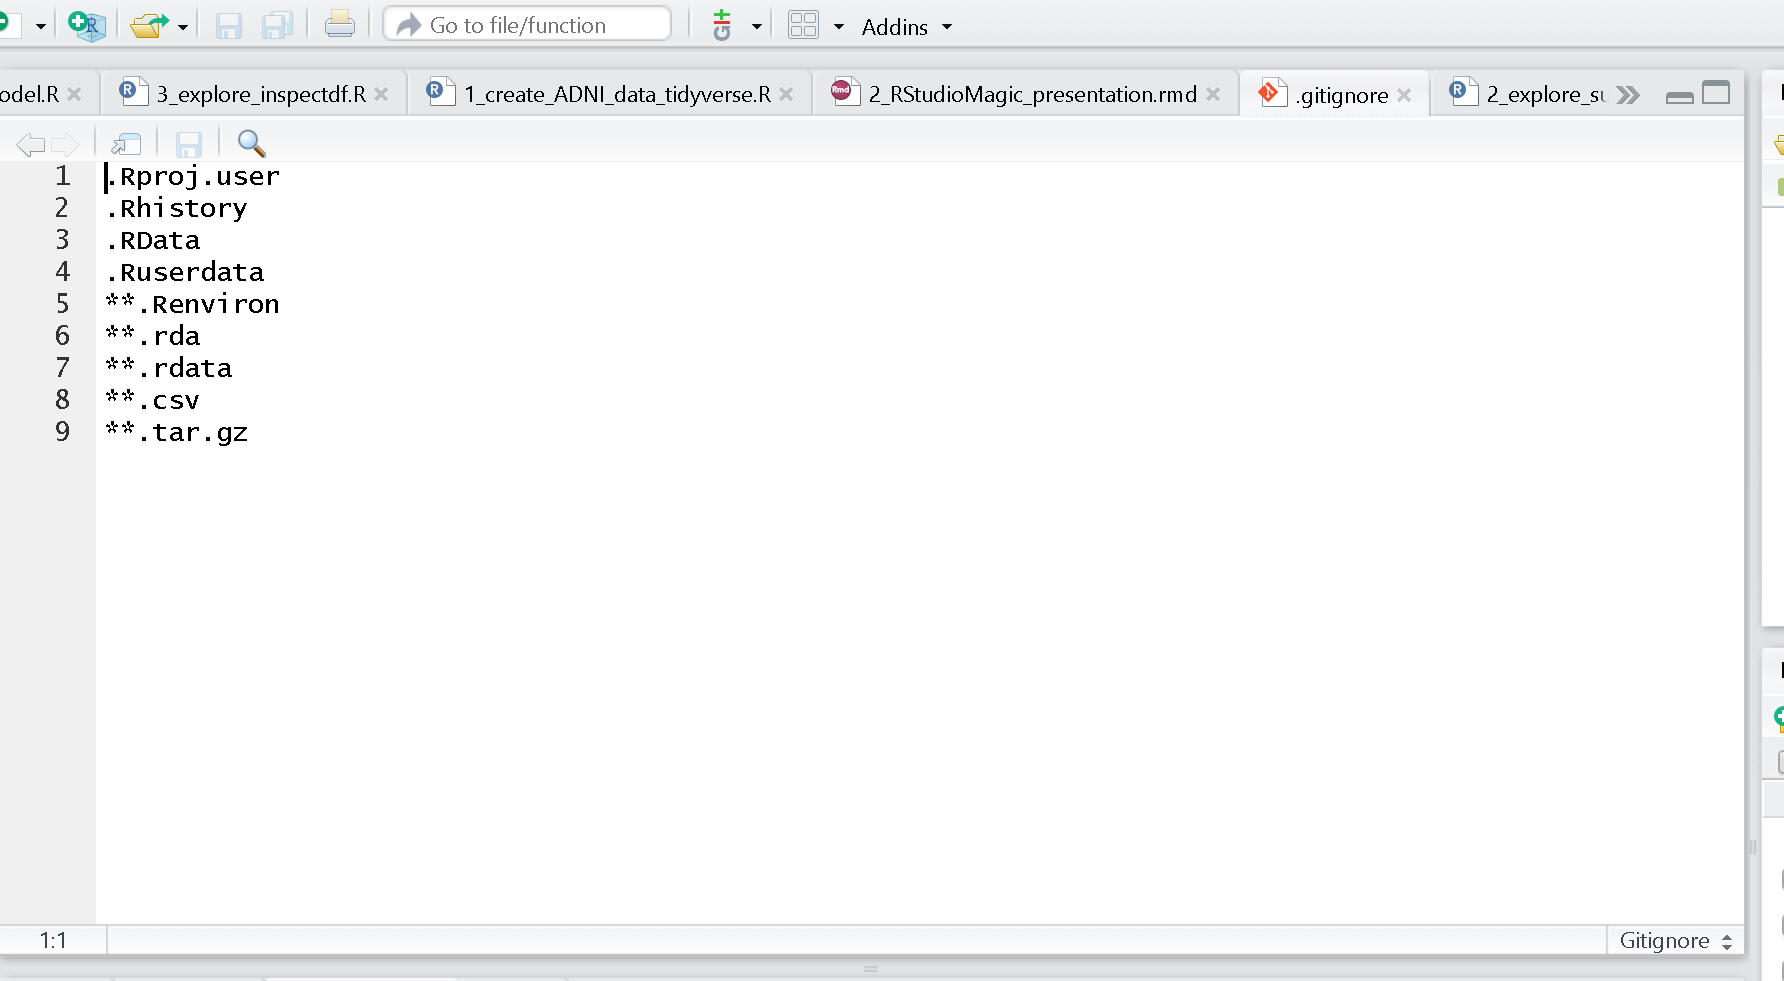
\includegraphics[width=0.75\textwidth,height=\textheight]{../external/images/gitignore.PNG}

\end{frame}

\end{document}
